\documentclass[12pt]{report}
\input{../bayesuvius.sty}
\begin{document}


Let

$N=$  number of branches
that each branch splits into, number of pieces that each piece breaks into.

$b=$ length (not area or volume) of initial piece
divided by length of final piece

$D=$ fractal dimension, $D>0$ can be less or more than one.

\beq
b^D = N, \quad D = \frac{\ln N}{\ln b}
\eeq

examples:
\begin{itemize}
\item line segment




\item square


\item Cantor set



\end{itemize}

\begin{figure}[h!]
\centering
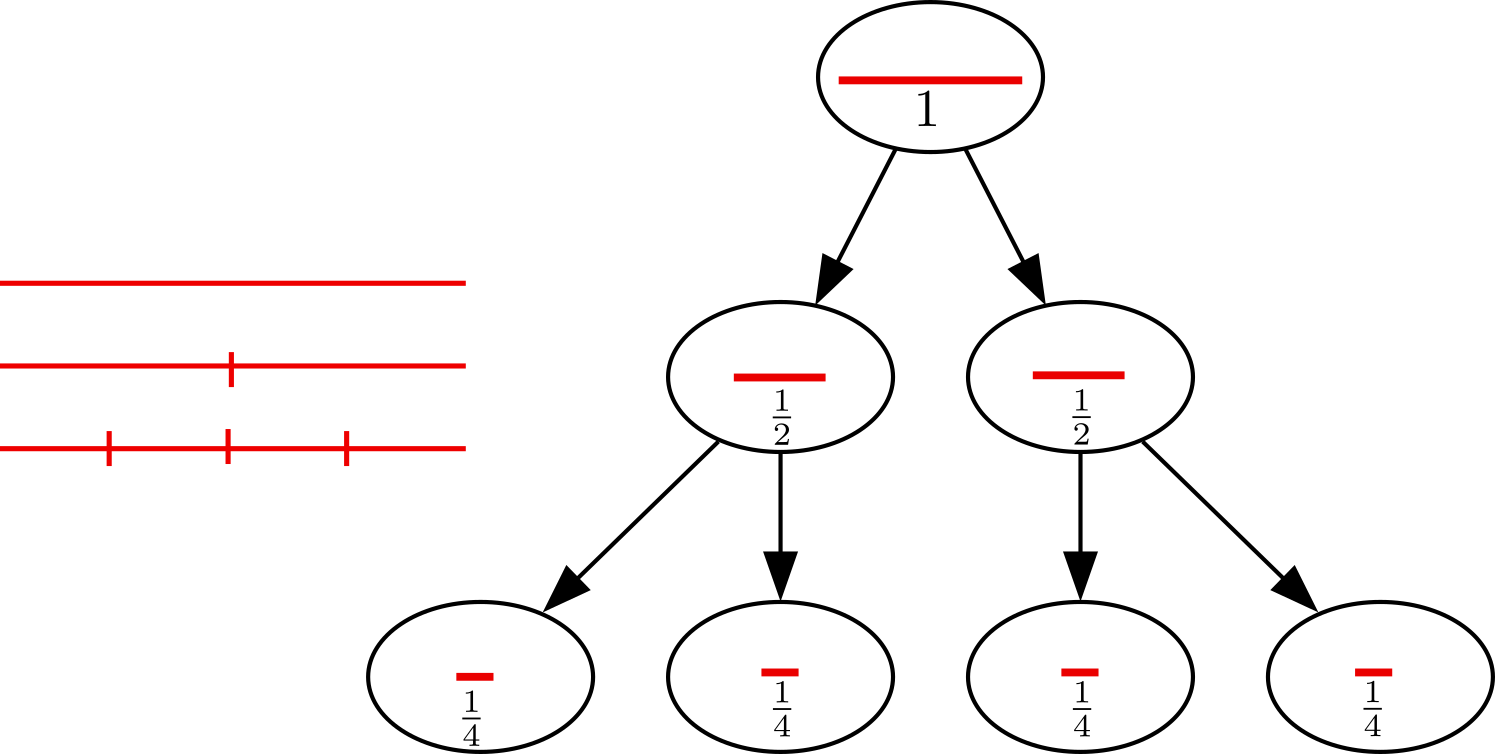
\includegraphics[width=5in]{line-segment.png}
\caption{View of Mount Vesuvius from
  Pompeii}
\label{fig-line-segment}
\end{figure}

\begin{figure}[h!]
\centering
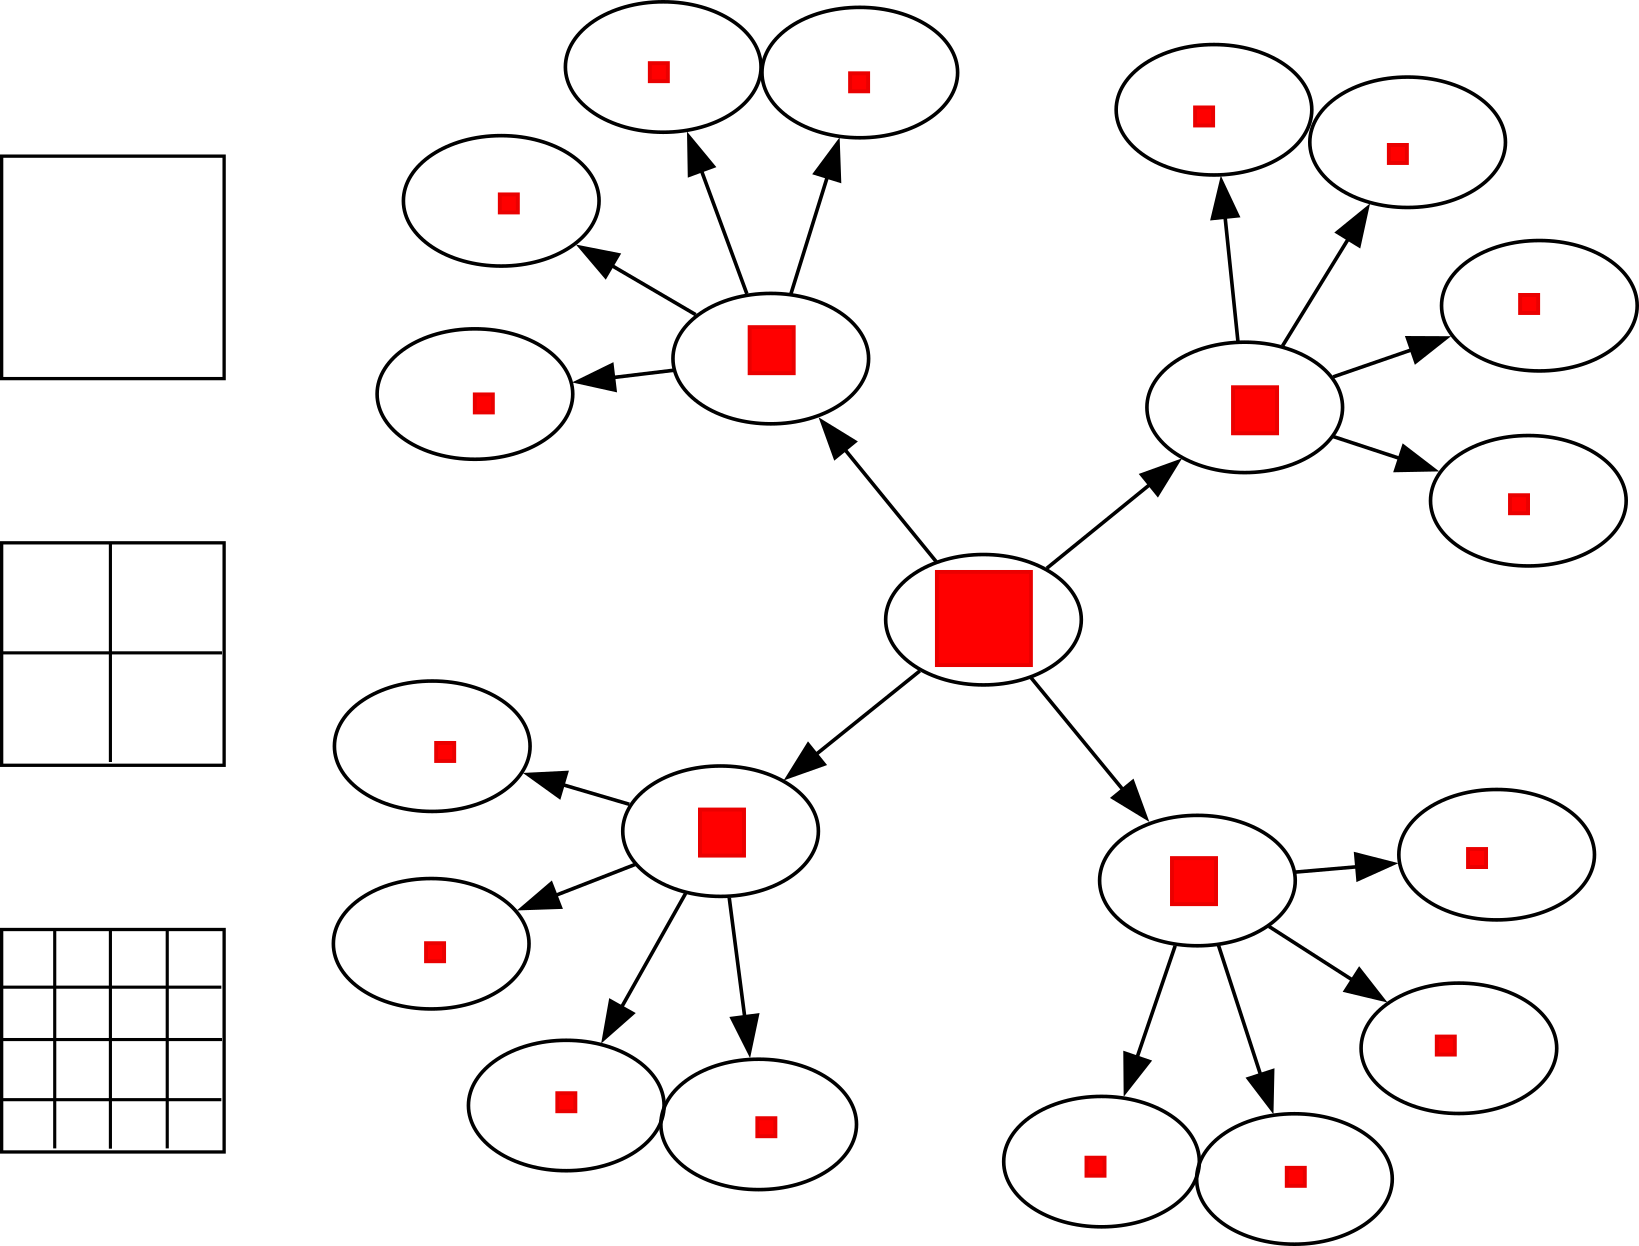
\includegraphics[width=5in]{square.png}
\caption{View of Mount Vesuvius from
  Pompeii}
\label{fig-square}
\end{figure}

\begin{figure}[h!]
\centering
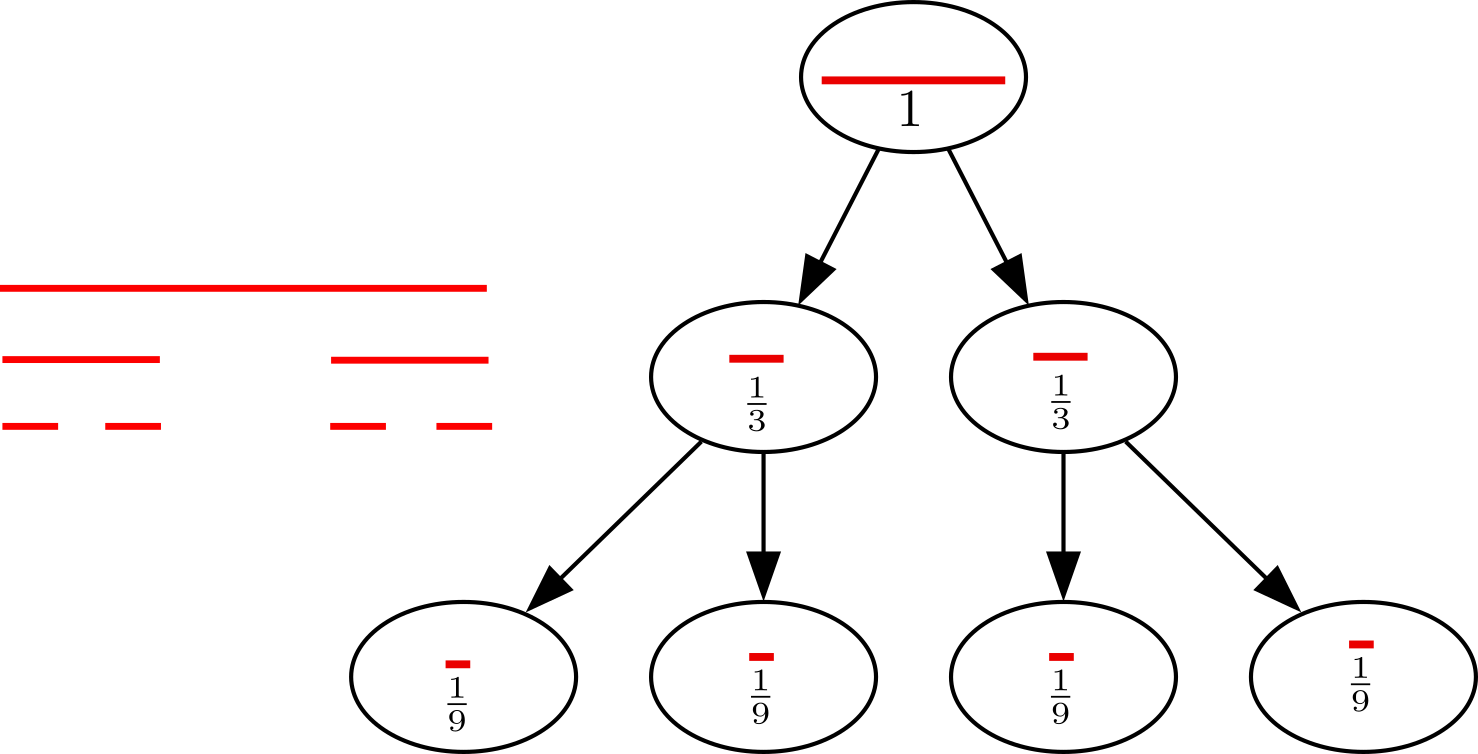
\includegraphics[width=5in]{cantor-set.png}
\caption{View of Mount Vesuvius from
  Pompeii}
\label{fig-cantor-set}
\end{figure}

\end{document}